\documentclass[1p]{elsarticle_modified}
%\bibliographystyle{elsarticle-num}

%\usepackage[colorlinks]{hyperref}
%\usepackage{abbrmath_seonhwa} %\Abb, \Ascr, \Acal ,\Abf, \Afrak
\usepackage{amsfonts}
\usepackage{amssymb}
\usepackage{amsmath}
\usepackage{amsthm}
\usepackage{scalefnt}
\usepackage{amsbsy}
\usepackage{kotex}
\usepackage{caption}
\usepackage{subfig}
\usepackage{color}
\usepackage{graphicx}
\usepackage{xcolor} %% white, black, red, green, blue, cyan, magenta, yellow
\usepackage{float}
\usepackage{setspace}
\usepackage{hyperref}

\usepackage{tikz}
\usetikzlibrary{arrows}

\usepackage{multirow}
\usepackage{array} % fixed length table
\usepackage{hhline}

%%%%%%%%%%%%%%%%%%%%%
\makeatletter
\renewcommand*\env@matrix[1][\arraystretch]{%
	\edef\arraystretch{#1}%
	\hskip -\arraycolsep
	\let\@ifnextchar\new@ifnextchar
	\array{*\c@MaxMatrixCols c}}
\makeatother %https://tex.stackexchange.com/questions/14071/how-can-i-increase-the-line-spacing-in-a-matrix
%%%%%%%%%%%%%%%

\usepackage[normalem]{ulem}

\newcommand{\msout}[1]{\ifmmode\text{\sout{\ensuremath{#1}}}\else\sout{#1}\fi}
%SOURCE: \msout is \stkout macro in https://tex.stackexchange.com/questions/20609/strikeout-in-math-mode

\newcommand{\cancel}[1]{
	\ifmmode
	{\color{red}\msout{#1}}
	\else
	{\color{red}\sout{#1}}
	\fi
}

\newcommand{\add}[1]{
	{\color{blue}\uwave{#1}}
}

\newcommand{\replace}[2]{
	\ifmmode
	{\color{red}\msout{#1}}{\color{blue}\uwave{#2}}
	\else
	{\color{red}\sout{#1}}{\color{blue}\uwave{#2}}
	\fi
}

\newcommand{\Sol}{\mathcal{S}} %segment
\newcommand{\D}{D} %diagram
\newcommand{\A}{\mathcal{A}} %arc


%%%%%%%%%%%%%%%%%%%%%%%%%%%%%5 test

\def\sl{\operatorname{\textup{SL}}(2,\Cbb)}
\def\psl{\operatorname{\textup{PSL}}(2,\Cbb)}
\def\quan{\mkern 1mu \triangleright \mkern 1mu}

\theoremstyle{definition}
\newtheorem{thm}{Theorem}[section]
\newtheorem{prop}[thm]{Proposition}
\newtheorem{lem}[thm]{Lemma}
\newtheorem{ques}[thm]{Question}
\newtheorem{cor}[thm]{Corollary}
\newtheorem{defn}[thm]{Definition}
\newtheorem{exam}[thm]{Example}
\newtheorem{rmk}[thm]{Remark}
\newtheorem{alg}[thm]{Algorithm}

\newcommand{\I}{\sqrt{-1}}
\begin{document}

%\begin{frontmatter}
%
%\title{Boundary parabolic representations of knots up to 8 crossings}
%
%%% Group authors per affiliation:
%\author{Yunhi Cho} 
%\address{Department of Mathematics, University of Seoul, Seoul, Korea}
%\ead{yhcho@uos.ac.kr}
%
%
%\author{Seonhwa Kim} %\fnref{s_kim}}
%\address{Center for Geometry and Physics, Institute for Basic Science, Pohang, 37673, Korea}
%\ead{ryeona17@ibs.re.kr}
%
%\author{Hyuk Kim}
%\address{Department of Mathematical Sciences, Seoul National University, Seoul 08826, Korea}
%\ead{hyukkim@snu.ac.kr}
%
%\author{Seokbeom Yoon}
%\address{Department of Mathematical Sciences, Seoul National University, Seoul, 08826,  Korea}
%\ead{sbyoon15@snu.ac.kr}
%
%\begin{abstract}
%We find all boundary parabolic representation of knots up to 8 crossings.
%
%\end{abstract}
%\begin{keyword}
%    \MSC[2010] 57M25 
%\end{keyword}
%
%\end{frontmatter}

%\linenumbers
%\tableofcontents
%
\newcommand\colored[1]{\textcolor{white}{\rule[-0.35ex]{0.8em}{1.4ex}}\kern-0.8em\color{red} #1}%
%\newcommand\colored[1]{\textcolor{white}{ #1}\kern-2.17ex	\textcolor{white}{ #1}\kern-1.81ex	\textcolor{white}{ #1}\kern-2.15ex\color{red}#1	}

{\Large $\underline{12a_{0519}~(K12a_{0519})}$}

\setlength{\tabcolsep}{10pt}
\renewcommand{\arraystretch}{1.6}
\vspace{1cm}\begin{tabular}{m{100pt}>{\centering\arraybackslash}m{274pt}}
\multirow{5}{120pt}{
	\centering
	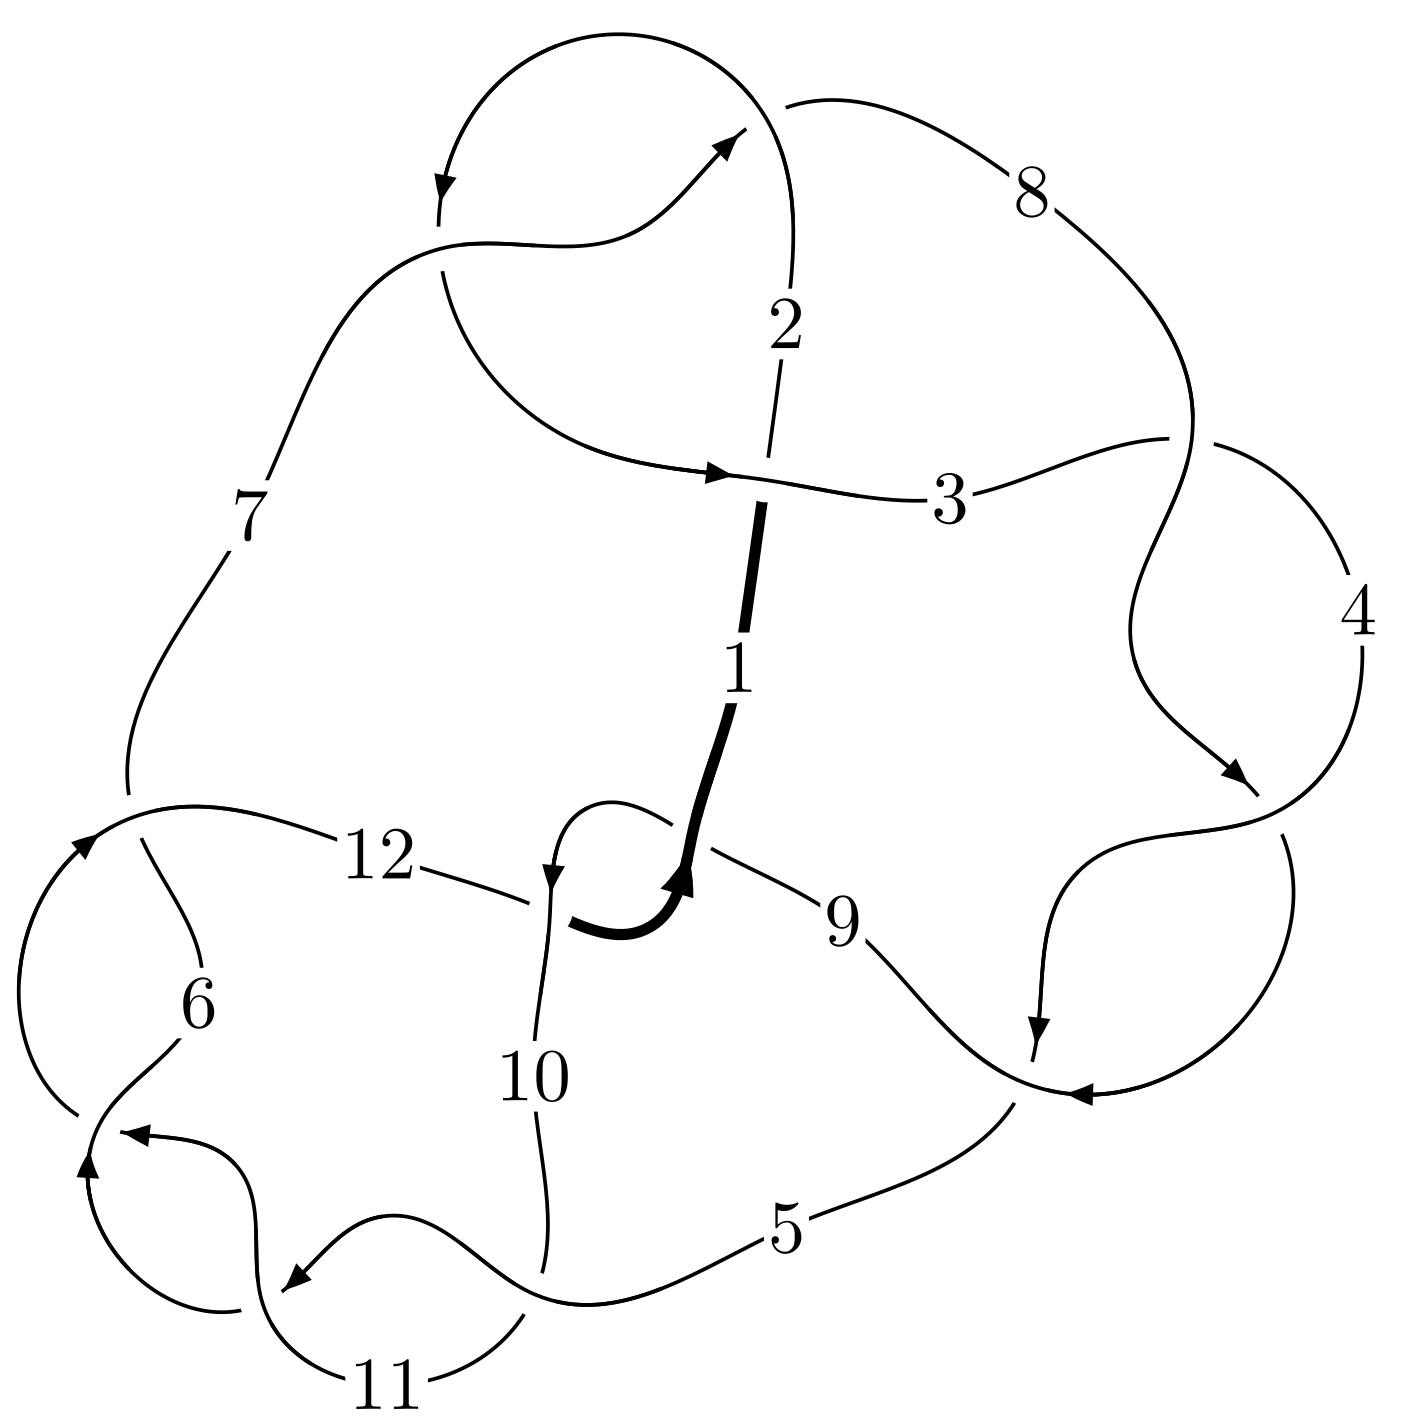
\includegraphics[width=112pt]{../../../GIT/diagram.site/Diagrams/png/1320_12a_0519.png}\\
\ \ \ A knot diagram\footnotemark}&
\allowdisplaybreaks
\textbf{Linearized knot diagam} \\
\cline{2-2}
 &
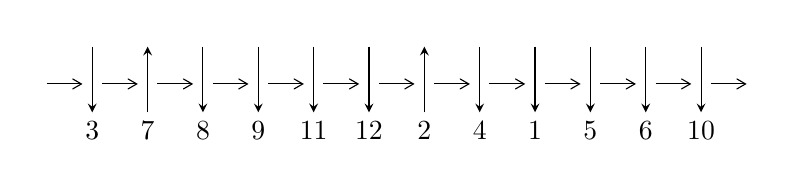
\begin{tikzpicture}[x=20pt, y=17pt]
	% nodes
	\node (C0) at (0, 0) {};
	\node (C1) at (1, 0) {};
	\node (C1U) at (1, +1) {};
	\node (C1D) at (1, -1) {3};

	\node (C2) at (2, 0) {};
	\node (C2U) at (2, +1) {};
	\node (C2D) at (2, -1) {7};

	\node (C3) at (3, 0) {};
	\node (C3U) at (3, +1) {};
	\node (C3D) at (3, -1) {8};

	\node (C4) at (4, 0) {};
	\node (C4U) at (4, +1) {};
	\node (C4D) at (4, -1) {9};

	\node (C5) at (5, 0) {};
	\node (C5U) at (5, +1) {};
	\node (C5D) at (5, -1) {11};

	\node (C6) at (6, 0) {};
	\node (C6U) at (6, +1) {};
	\node (C6D) at (6, -1) {12};

	\node (C7) at (7, 0) {};
	\node (C7U) at (7, +1) {};
	\node (C7D) at (7, -1) {2};

	\node (C8) at (8, 0) {};
	\node (C8U) at (8, +1) {};
	\node (C8D) at (8, -1) {4};

	\node (C9) at (9, 0) {};
	\node (C9U) at (9, +1) {};
	\node (C9D) at (9, -1) {1};

	\node (C10) at (10, 0) {};
	\node (C10U) at (10, +1) {};
	\node (C10D) at (10, -1) {5};

	\node (C11) at (11, 0) {};
	\node (C11U) at (11, +1) {};
	\node (C11D) at (11, -1) {6};

	\node (C12) at (12, 0) {};
	\node (C12U) at (12, +1) {};
	\node (C12D) at (12, -1) {10};
	\node (C13) at (13, 0) {};

	% arrows
	\draw[->,>={angle 60}]
	(C0) edge (C1) (C1) edge (C2) (C2) edge (C3) (C3) edge (C4) (C4) edge (C5) (C5) edge (C6) (C6) edge (C7) (C7) edge (C8) (C8) edge (C9) (C9) edge (C10) (C10) edge (C11) (C11) edge (C12) (C12) edge (C13) ;	\draw[->,>=stealth]
	(C1U) edge (C1D) (C2D) edge (C2U) (C3U) edge (C3D) (C4U) edge (C4D) (C5U) edge (C5D) (C6U) edge (C6D) (C7D) edge (C7U) (C8U) edge (C8D) (C9U) edge (C9D) (C10U) edge (C10D) (C11U) edge (C11D) (C12U) edge (C12D) ;
	\end{tikzpicture} \\
\hhline{~~} \\& 
\textbf{Solving Sequence} \\ \cline{2-2} 
 &
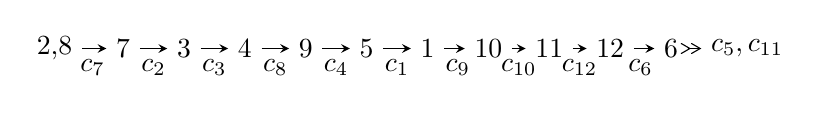
\begin{tikzpicture}[x=22pt, y=7pt]
	% node
	\node (A0) at (-1/8, 0) {2,8};
	\node (A1) at (1, 0) {7};
	\node (A2) at (2, 0) {3};
	\node (A3) at (3, 0) {4};
	\node (A4) at (4, 0) {9};
	\node (A5) at (5, 0) {5};
	\node (A6) at (6, 0) {1};
	\node (A7) at (7, 0) {10};
	\node (A8) at (8, 0) {11};
	\node (A9) at (9, 0) {12};
	\node (A10) at (10, 0) {6};
	\node (C1) at (1/2, -1) {$c_{7}$};
	\node (C2) at (3/2, -1) {$c_{2}$};
	\node (C3) at (5/2, -1) {$c_{3}$};
	\node (C4) at (7/2, -1) {$c_{8}$};
	\node (C5) at (9/2, -1) {$c_{4}$};
	\node (C6) at (11/2, -1) {$c_{1}$};
	\node (C7) at (13/2, -1) {$c_{9}$};
	\node (C8) at (15/2, -1) {$c_{10}$};
	\node (C9) at (17/2, -1) {$c_{12}$};
	\node (C10) at (19/2, -1) {$c_{6}$};
	\node (A11) at (45/4, 0) {$c_{5},c_{11}$};

	% edge
	\draw[->,>=stealth]	
	(A0) edge (A1) (A1) edge (A2) (A2) edge (A3) (A3) edge (A4) (A4) edge (A5) (A5) edge (A6) (A6) edge (A7) (A7) edge (A8) (A8) edge (A9) (A9) edge (A10) ;
	\draw[->>,>={angle 60}]	
	(A10) edge (A11);
\end{tikzpicture} \\ 

\end{tabular} \\

\footnotetext{
The image of knot diagram is generated by the software ``\textbf{Draw programme}" developed by Andrew Bartholomew(\url{http://www.layer8.co.uk/maths/draw/index.htm\#Running-draw}), where we modified some parts for our purpose(\url{https://github.com/CATsTAILs/LinksPainter}).
}\phantom \\ \newline 
\centering \textbf{Ideals for irreducible components\footnotemark of $X_{\text{par}}$} 
 
\begin{align*}
I^u_{1}&=\langle 
u^{55}+u^{54}+\cdots-2 u-1\rangle \\
\\
\end{align*}
\raggedright * 1 irreducible components of $\dim_{\mathbb{C}}=0$, with total 55 representations.\\
\footnotetext{All coefficients of polynomials are rational numbers. But the coefficients are sometimes approximated in decimal forms when there is not enough margin.}
\newpage
\renewcommand{\arraystretch}{1}
\centering \section*{I. $I^u_{1}= \langle u^{55}+u^{54}+\cdots-2 u-1 \rangle$}
\flushleft \textbf{(i) Arc colorings}\\
\begin{tabular}{m{7pt} m{180pt} m{7pt} m{180pt} }
\flushright $a_{2}=$&$\begin{pmatrix}0\\u\end{pmatrix}$ \\
\flushright $a_{8}=$&$\begin{pmatrix}1\\0\end{pmatrix}$ \\
\flushright $a_{7}=$&$\begin{pmatrix}1\\u^2\end{pmatrix}$ \\
\flushright $a_{3}=$&$\begin{pmatrix}u\\u^3+u\end{pmatrix}$ \\
\flushright $a_{4}=$&$\begin{pmatrix}- u^3\\u^3+u\end{pmatrix}$ \\
\flushright $a_{9}=$&$\begin{pmatrix}- u^6- u^4+1\\u^6+2 u^4+u^2\end{pmatrix}$ \\
\flushright $a_{5}=$&$\begin{pmatrix}u^9+2 u^7+u^5-2 u^3- u\\- u^9-3 u^7-3 u^5+u\end{pmatrix}$ \\
\flushright $a_{1}=$&$\begin{pmatrix}u^3\\u^5+u^3+u\end{pmatrix}$ \\
\flushright $a_{10}=$&$\begin{pmatrix}- u^{14}-3 u^{12}-4 u^{10}- u^8+1\\- u^{16}-4 u^{14}-8 u^{12}-8 u^{10}-4 u^8+2 u^6+4 u^4+2 u^2\end{pmatrix}$ \\
\flushright $a_{11}=$&$\begin{pmatrix}u^{34}+9 u^{32}+\cdots- u^2+1\\- u^{34}-10 u^{32}+\cdots+6 u^4+3 u^2\end{pmatrix}$ \\
\flushright $a_{12}=$&$\begin{pmatrix}u^{25}+6 u^{23}+\cdots+2 u^3+u\\u^{27}+7 u^{25}+\cdots+3 u^3+u\end{pmatrix}$ \\
\flushright $a_{6}=$&$\begin{pmatrix}- u^{50}-13 u^{48}+\cdots- u^2+1\\- u^{52}-14 u^{50}+\cdots-18 u^6-5 u^4\end{pmatrix}$\\&\end{tabular}
\flushleft \textbf{(ii) Obstruction class $= -1$}\\~\\
\flushleft \textbf{(iii) Cusp Shapes $= 4 u^{53}+4 u^{52}+\cdots-4 u-14$}\\~\\
\newpage\renewcommand{\arraystretch}{1}
\flushleft \textbf{(iv) u-Polynomials at the component}\newline \\
\begin{tabular}{m{50pt}|m{274pt}}
Crossings & \hspace{64pt}u-Polynomials at each crossing \\
\hline $$\begin{aligned}c_{1}\end{aligned}$$&$\begin{aligned}
&u^{55}+31 u^{54}+\cdots+4 u-1
\end{aligned}$\\
\hline $$\begin{aligned}c_{2},c_{7}\end{aligned}$$&$\begin{aligned}
&u^{55}+u^{54}+\cdots-2 u-1
\end{aligned}$\\
\hline $$\begin{aligned}c_{3},c_{4},c_{8}\end{aligned}$$&$\begin{aligned}
&u^{55}- u^{54}+\cdots+u-2
\end{aligned}$\\
\hline $$\begin{aligned}c_{5},c_{6},c_{10}\\c_{11}\end{aligned}$$&$\begin{aligned}
&u^{55}+u^{54}+\cdots-2 u-1
\end{aligned}$\\
\hline $$\begin{aligned}c_{9},c_{12}\end{aligned}$$&$\begin{aligned}
&u^{55}-11 u^{54}+\cdots+8 u-1
\end{aligned}$\\
\hline
\end{tabular}\\~\\
\newpage\renewcommand{\arraystretch}{1}
\flushleft \textbf{(v) Riley Polynomials at the component}\newline \\
\begin{tabular}{m{50pt}|m{274pt}}
Crossings & \hspace{64pt}Riley Polynomials at each crossing \\
\hline $$\begin{aligned}c_{1}\end{aligned}$$&$\begin{aligned}
&y^{55}-13 y^{54}+\cdots+68 y-1
\end{aligned}$\\
\hline $$\begin{aligned}c_{2},c_{7}\end{aligned}$$&$\begin{aligned}
&y^{55}+31 y^{54}+\cdots+4 y-1
\end{aligned}$\\
\hline $$\begin{aligned}c_{3},c_{4},c_{8}\end{aligned}$$&$\begin{aligned}
&y^{55}-57 y^{54}+\cdots+293 y-4
\end{aligned}$\\
\hline $$\begin{aligned}c_{5},c_{6},c_{10}\\c_{11}\end{aligned}$$&$\begin{aligned}
&y^{55}-61 y^{54}+\cdots+4 y-1
\end{aligned}$\\
\hline $$\begin{aligned}c_{9},c_{12}\end{aligned}$$&$\begin{aligned}
&y^{55}+23 y^{54}+\cdots-36 y-1
\end{aligned}$\\
\hline
\end{tabular}\\~\\
\newpage\flushleft \textbf{(vi) Complex Volumes and Cusp Shapes}
$$\begin{array}{c|c|c}  
\text{Solutions to }I^u_{1}& \I (\text{vol} + \sqrt{-1}CS) & \text{Cusp shape}\\
 \hline 
\begin{aligned}
u &= -0.102308 + 0.993927 I\end{aligned}
 & -1.51781 + 1.35357 I & -14.4750 - 4.2304 I \\ \hline\begin{aligned}
u &= -0.102308 - 0.993927 I\end{aligned}
 & -1.51781 - 1.35357 I & -14.4750 + 4.2304 I \\ \hline\begin{aligned}
u &= -0.485253 + 0.877654 I\end{aligned}
 & -4.60903 - 0.50394 I & -9.84299 + 3.20622 I \\ \hline\begin{aligned}
u &= -0.485253 - 0.877654 I\end{aligned}
 & -4.60903 + 0.50394 I & -9.84299 - 3.20622 I \\ \hline\begin{aligned}
u &= \phantom{-}0.479095 + 0.928930 I\end{aligned}
 & \phantom{-}1.53724 + 2.73421 I & -6.40413 - 2.99488 I \\ \hline\begin{aligned}
u &= \phantom{-}0.479095 - 0.928930 I\end{aligned}
 & \phantom{-}1.53724 - 2.73421 I & -6.40413 + 2.99488 I \\ \hline\begin{aligned}
u &= -0.328532 + 0.998033 I\end{aligned}
 & -3.02866 - 2.73775 I & -17.4070 + 6.3920 I \\ \hline\begin{aligned}
u &= -0.328532 - 0.998033 I\end{aligned}
 & -3.02866 + 2.73775 I & -17.4070 - 6.3920 I \\ \hline\begin{aligned}
u &= \phantom{-}0.116890 + 1.065220 I\end{aligned}
 & -8.61843 - 3.30249 I & -17.5441 + 2.1403 I \\ \hline\begin{aligned}
u &= \phantom{-}0.116890 - 1.065220 I\end{aligned}
 & -8.61843 + 3.30249 I & -17.5441 - 2.1403 I \\ \hline\begin{aligned}
u &= -0.491393 + 0.960867 I\end{aligned}
 & \phantom{-}1.09428 - 6.52024 I & -8.28646 + 9.91432 I \\ \hline\begin{aligned}
u &= -0.491393 - 0.960867 I\end{aligned}
 & \phantom{-}1.09428 + 6.52024 I & -8.28646 - 9.91432 I \\ \hline\begin{aligned}
u &= \phantom{-}0.503891 + 0.983618 I\end{aligned}
 & -5.90815 + 9.04807 I & -12.0898 - 8.5316 I \\ \hline\begin{aligned}
u &= \phantom{-}0.503891 - 0.983618 I\end{aligned}
 & -5.90815 - 9.04807 I & -12.0898 + 8.5316 I \\ \hline\begin{aligned}
u &= \phantom{-}0.243423 + 0.854516 I\end{aligned}
 & -0.623812 + 1.209860 I & -7.64614 - 4.90268 I \\ \hline\begin{aligned}
u &= \phantom{-}0.243423 - 0.854516 I\end{aligned}
 & -0.623812 - 1.209860 I & -7.64614 + 4.90268 I \\ \hline\begin{aligned}
u &= -0.870822\phantom{ +0.000000I}\end{aligned}
 & -14.9278\phantom{ +0.000000I} & -15.7210\phantom{ +0.000000I} \\ \hline\begin{aligned}
u &= \phantom{-}0.333283 + 1.082310 I\end{aligned}
 & -10.49970 + 3.34960 I & -17.9466 - 4.0527 I \\ \hline\begin{aligned}
u &= \phantom{-}0.333283 - 1.082310 I\end{aligned}
 & -10.49970 - 3.34960 I & -17.9466 + 4.0527 I \\ \hline\begin{aligned}
u &= -0.861168 + 0.072729 I\end{aligned}
 & -10.59330 + 8.29227 I & -12.98061 - 4.57740 I \\ \hline\begin{aligned}
u &= -0.861168 - 0.072729 I\end{aligned}
 & -10.59330 - 8.29227 I & -12.98061 + 4.57740 I \\ \hline\begin{aligned}
u &= \phantom{-}0.845961 + 0.068541 I\end{aligned}
 & -3.20212 - 5.70812 I & -9.97360 + 5.97545 I \\ \hline\begin{aligned}
u &= \phantom{-}0.845961 - 0.068541 I\end{aligned}
 & -3.20212 + 5.70812 I & -9.97360 - 5.97545 I \\ \hline\begin{aligned}
u &= \phantom{-}0.840103\phantom{ +0.000000I}\end{aligned}
 & -6.53703\phantom{ +0.000000I} & -14.4920\phantom{ +0.000000I} \\ \hline\begin{aligned}
u &= -0.825031 + 0.057929 I\end{aligned}
 & -2.24307 + 1.86074 I & -7.46523 + 0.06131 I \\ \hline\begin{aligned}
u &= -0.825031 - 0.057929 I\end{aligned}
 & -2.24307 - 1.86074 I & -7.46523 - 0.06131 I \\ \hline\begin{aligned}
u &= -0.514519 + 0.590131 I\end{aligned}
 & -3.81103 - 3.61233 I & -7.78381 + 3.89227 I \\ \hline\begin{aligned}
u &= -0.514519 - 0.590131 I\end{aligned}
 & -3.81103 + 3.61233 I & -7.78381 - 3.89227 I \\ \hline\begin{aligned}
u &= \phantom{-}0.503991 + 0.523196 I\end{aligned}
 & \phantom{-}2.66446 + 1.32817 I & -3.49967 - 4.01662 I \\ \hline\begin{aligned}
u &= \phantom{-}0.503991 - 0.523196 I\end{aligned}
 & \phantom{-}2.66446 - 1.32817 I & -3.49967 + 4.01662 I\\
 \hline 
 \end{array}$$\newpage$$\begin{array}{c|c|c}  
\text{Solutions to }I^u_{1}& \I (\text{vol} + \sqrt{-1}CS) & \text{Cusp shape}\\
 \hline 
\begin{aligned}
u &= \phantom{-}0.726197\phantom{ +0.000000I}\end{aligned}
 & -7.37532\phantom{ +0.000000I} & -11.5790\phantom{ +0.000000I} \\ \hline\begin{aligned}
u &= \phantom{-}0.572655 + 0.425482 I\end{aligned}
 & -4.35800 - 4.75776 I & -8.70806 + 3.36680 I \\ \hline\begin{aligned}
u &= \phantom{-}0.572655 - 0.425482 I\end{aligned}
 & -4.35800 + 4.75776 I & -8.70806 - 3.36680 I \\ \hline\begin{aligned}
u &= \phantom{-}0.463308 + 1.201860 I\end{aligned}
 & -10.77920 + 4.40954 I & \phantom{-0.000000 } 0 \\ \hline\begin{aligned}
u &= \phantom{-}0.463308 - 1.201860 I\end{aligned}
 & -10.77920 - 4.40954 I & \phantom{-0.000000 } 0 \\ \hline\begin{aligned}
u &= -0.530920 + 0.462145 I\end{aligned}
 & \phantom{-}2.47339 + 2.35970 I & -4.46729 - 4.22291 I \\ \hline\begin{aligned}
u &= -0.530920 - 0.462145 I\end{aligned}
 & \phantom{-}2.47339 - 2.35970 I & -4.46729 + 4.22291 I \\ \hline\begin{aligned}
u &= -0.431213 + 1.227700 I\end{aligned}
 & -6.07588 - 2.53923 I & \phantom{-0.000000 } 0 \\ \hline\begin{aligned}
u &= -0.431213 - 1.227700 I\end{aligned}
 & -6.07588 + 2.53923 I & \phantom{-0.000000 } 0 \\ \hline\begin{aligned}
u &= \phantom{-}0.423975 + 1.239910 I\end{aligned}
 & -7.15358 - 1.27519 I & \phantom{-0.000000 } 0 \\ \hline\begin{aligned}
u &= \phantom{-}0.423975 - 1.239910 I\end{aligned}
 & -7.15358 + 1.27519 I & \phantom{-0.000000 } 0 \\ \hline\begin{aligned}
u &= -0.485017 + 1.219700 I\end{aligned}
 & -5.68867 - 6.60293 I & \phantom{-0.000000 } 0 \\ \hline\begin{aligned}
u &= -0.485017 - 1.219700 I\end{aligned}
 & -5.68867 + 6.60293 I & \phantom{-0.000000 } 0 \\ \hline\begin{aligned}
u &= \phantom{-}0.459979 + 1.232640 I\end{aligned}
 & -10.22260 + 4.63419 I & \phantom{-0.000000 } 0 \\ \hline\begin{aligned}
u &= \phantom{-}0.459979 - 1.232640 I\end{aligned}
 & -10.22260 - 4.63419 I & \phantom{-0.000000 } 0 \\ \hline\begin{aligned}
u &= -0.421595 + 1.249750 I\end{aligned}
 & -14.6184 + 3.8161 I & \phantom{-0.000000 } 0 \\ \hline\begin{aligned}
u &= -0.421595 - 1.249750 I\end{aligned}
 & -14.6184 - 3.8161 I & \phantom{-0.000000 } 0 \\ \hline\begin{aligned}
u &= \phantom{-}0.492780 + 1.225990 I\end{aligned}
 & -6.65767 + 10.54660 I & \phantom{-0.000000 } 0 \\ \hline\begin{aligned}
u &= \phantom{-}0.492780 - 1.225990 I\end{aligned}
 & -6.65767 - 10.54660 I & \phantom{-0.000000 } 0 \\ \hline\begin{aligned}
u &= -0.497583 + 1.231530 I\end{aligned}
 & -14.0678 - 13.1961 I & \phantom{-0.000000 } 0 \\ \hline\begin{aligned}
u &= -0.497583 - 1.231530 I\end{aligned}
 & -14.0678 + 13.1961 I & \phantom{-0.000000 } 0 \\ \hline\begin{aligned}
u &= -0.464095 + 1.248480 I\end{aligned}
 & -18.7025 - 4.7501 I & \phantom{-0.000000 } 0 \\ \hline\begin{aligned}
u &= -0.464095 - 1.248480 I\end{aligned}
 & -18.7025 + 4.7501 I & \phantom{-0.000000 } 0 \\ \hline\begin{aligned}
u &= \phantom{-}0.653534\phantom{ +0.000000I}\end{aligned}
 & -7.36372\phantom{ +0.000000I} & -12.0180\phantom{ +0.000000I} \\ \hline\begin{aligned}
u &= -0.350221\phantom{ +0.000000I}\end{aligned}
 & -0.718328\phantom{ +0.000000I} & -13.6840\phantom{ +0.000000I}\\
 \hline 
 \end{array}$$\newpage
\newpage\renewcommand{\arraystretch}{1}
\centering \section*{ II. u-Polynomials}
\begin{tabular}{m{50pt}|m{274pt}}
Crossings & \hspace{64pt}u-Polynomials at each crossing \\
\hline $$\begin{aligned}c_{1}\end{aligned}$$&$\begin{aligned}
&u^{55}+31 u^{54}+\cdots+4 u-1
\end{aligned}$\\
\hline $$\begin{aligned}c_{2},c_{7}\end{aligned}$$&$\begin{aligned}
&u^{55}+u^{54}+\cdots-2 u-1
\end{aligned}$\\
\hline $$\begin{aligned}c_{3},c_{4},c_{8}\end{aligned}$$&$\begin{aligned}
&u^{55}- u^{54}+\cdots+u-2
\end{aligned}$\\
\hline $$\begin{aligned}c_{5},c_{6},c_{10}\\c_{11}\end{aligned}$$&$\begin{aligned}
&u^{55}+u^{54}+\cdots-2 u-1
\end{aligned}$\\
\hline $$\begin{aligned}c_{9},c_{12}\end{aligned}$$&$\begin{aligned}
&u^{55}-11 u^{54}+\cdots+8 u-1
\end{aligned}$\\
\hline
\end{tabular}\newpage\renewcommand{\arraystretch}{1}
\centering \section*{ III. Riley Polynomials}
\begin{tabular}{m{50pt}|m{274pt}}
Crossings & \hspace{64pt}Riley Polynomials at each crossing \\
\hline $$\begin{aligned}c_{1}\end{aligned}$$&$\begin{aligned}
&y^{55}-13 y^{54}+\cdots+68 y-1
\end{aligned}$\\
\hline $$\begin{aligned}c_{2},c_{7}\end{aligned}$$&$\begin{aligned}
&y^{55}+31 y^{54}+\cdots+4 y-1
\end{aligned}$\\
\hline $$\begin{aligned}c_{3},c_{4},c_{8}\end{aligned}$$&$\begin{aligned}
&y^{55}-57 y^{54}+\cdots+293 y-4
\end{aligned}$\\
\hline $$\begin{aligned}c_{5},c_{6},c_{10}\\c_{11}\end{aligned}$$&$\begin{aligned}
&y^{55}-61 y^{54}+\cdots+4 y-1
\end{aligned}$\\
\hline $$\begin{aligned}c_{9},c_{12}\end{aligned}$$&$\begin{aligned}
&y^{55}+23 y^{54}+\cdots-36 y-1
\end{aligned}$\\
\hline
\end{tabular}
\vskip 2pc
\end{document}